\chapter{Fairness} \label{chap:fairness}
% TODO: Introduction into the chapter, what we want to achieve, that we want try to define what Fairness is and how to measure it.

% TODO: Reword
So far, we have discussed recommender systems and the methods that are used in the field. But now, let us step back and look at the problem from a broader perspective of fairness as a social construct. Specifically, we will focus on the importance of fairness in the context of algorithms, what role it plays when using machine learning models with potentially sensitive data and see how and if we can make group recommenders better when we understand and define the underlying properties.

We will start with a general introduction to the topic of fairness, define its possible meanings and specify which one is important in our setting.
%\todo[inline]{vete chybi subject (we)}
This is required due to the overload of the word itself and the rising importance of the topic in today's world. Furthermore
%\todo[inline]{spis furthermore?}
, we will explain why fairness seems to be a crucial parameter in the group recommender setting and will try to reason about how to measure its effects.




\section{General} \label{sec:02_general}
% TODO: Start with a broad overview, why do we need something like fairness, define it, speak about it broadly.
% TODO: Problems with fairness, areas of usage, many possible definitions.

% I want to make an argument, that fairness is important to prevent notions of inequality which inherently leads to negative emotions

% it should lead the reader to think about it more, all the things we are discussing are general knowledge, we are not introducing something crazy

% IDEAS: Mention usage of the word fair/fairness
% https://www.youtube.com/watch?v=dKob6b8QzkU
% monkeys 
% https://www.youtube.com/watch?v=vHE6AYNOCrg
% many meaning of the word fairness, what does it mean for something to be fair

% the notion of fairness is probably important for developing cooperation

The word fairness
%\todo[inline]{pridal bych "fairness"}
itself is very hard and controversial to define.
%\todo[inline]{pridal bych carku}
In Cambridge Dictionary \cite{fairness_definition} it is
%\todo[inline]{zkracene is za 's se obecne nedoporucuje uvadet ve vedeckych textech - dobre pravidlo je ze apostroph je prijatelny jen u privlastnovacich vyrazu (John's shoe)}
defined as "The quality of treating people equally or in a way that is reasonable." Its use has been rising steadily from the 1960s as we can see on \ref{fig:popularity_of_fairness}.

\begin{figure}[htbp]
    \centering
    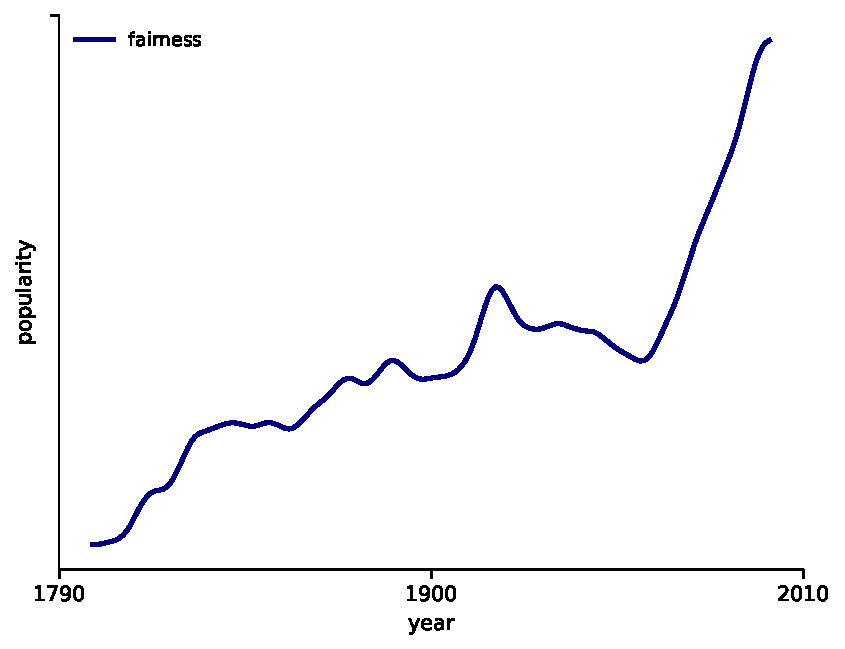
\includegraphics{img/google_ngram_fairness-eng_2012-1800-2000.pdf}
    \caption{The graph shows the phrase "fairness" occurring in the corpus of English books from 1800 to 2010. Source: Google Ngram Viewer, corpora 2012. \cite{google_ngram_viewer_2012}}
    \label{fig:popularity_of_fairness}
\end{figure}

Humans are obsessed with fairness. From a young age, children will get sad when something is not fair, when their sibling gets a more significant piece of a pie, more attention from their parent, or any other unequal situation. It can induce strong emotions such as envy, sadness, or anger, and it emerges very early, as early as 12 months of age or sooner as researched in \cite{children_fairness}.

And this behavior is not limited only to humans. We can observe the same behavior in monkeys. In \cite{brosnan2003monkeys}, the authors observed that if a monkey is getting the worse reward for the same task as its peer,  it refuses the reward and demands the same payout even if they were satisfied with the lesser reward for the same task before. In some sense, this is very strange, why should you care about someone having more if you have enough?

We observe the same behavior in many other species of animals, but not all. It seems that it requires a certain level of intelligence for the notion of fairness to emerge. As discussed in \cite{brosnan2014evolution}, based on studies of other non-human species, this evolutionary puzzle can be further dissected into responses to reward distribution among the cooperating group members. Where humans are willing to seek equalization of outcomes even if it means that they will loose some of their own reward as studied in \cite{willing_to_pay_to_equality}. At the same time, we humans like "free-rides" where we get high rewards for a small amount of work but dislike when someone else gets the same. This directly corresponds with the fairness itself - "It is not fair if someone else gets something we don't.". However, it all depends on our personality and the type of relationship involved. Some people are, for example, willing to accept that their partner makes more, but that is very subjective and in some cases can lead even to larger envy involved.

In some cases we observe a pattern of generosity, where children are willing to make their own sacrifices in order to ensure fairness, so that the other person does not have less than them, as presented in \cite{children_generocity_blake}. The authors studied fairness in multiple cultural settings and found out that this behavior is learned and only present in some cultures.

On the other hand, our society widely accepts the notion of "winner takes all", which can be problematic in itself, for example, in sports and business. In business it directly shapes the distribution of wealth, which is considered as one of the main problems of today's world. But discussing the social aspect of fairness is beyond the scope of this thesis.

When it comes to the true nature of fairness on the deepest level, it could even be possible that the notion of fairness emerges together with cooperation and therefore language and communication. It would mean that it is an inherent property of any intelligent agent that is created through an evolutionary process.
Another point of view could be that fairness acts as a mechanism that pushes towards equality among the group members and that leads to a higher stability of the group which would give an evolutionary advantage.
But more research has to be done, as our understanding of intelligence, consciousness, and related hard to quantify phenomena is lacking.\newline

Let us now get back to fairness in the context of computer systems.







\section{Algorithmic fairness}\label{subsec:02_general.algorithmic_fairness_and_possible_meanings}
% The Emerging Theory of Algorithmic Fairness
We will focus on fairness regarding society or individuals interacting with a computer system. We will not discuss further any meaning of fairness outside of the domain of computer science. This topic steers away from the main goal of defining fairness for the group RS sub-domain, but we think that it is very important topic in general, deserves more spotlight and can be a good middle step to understand specifics of the group RS setting.

\subsection{Sources of algorithmic unfairness}
%\todo[inline]{Pokud bys chtel neco formalnejsiho tak jako nadpis navrhuju Sources of algorithmic unfairness. Jinak ja bych tu variantu ze algoritmus je by design neferovy uplne nevyhazoval out of consideration. Treba cinsky credit score system - aneb je fer ze si nesmis koupit letenku protoze jsi prechazel na cervenou?}
%\todo[inline]{mozna radeji no understanding? Notion by mohl byt prosty fakt ze zna atribut}
%\todo[inline]{tahle veta je divna, chtelo by to lepe navazat - co  myslis tim ze autori algoritmu jsou lide - ze napsali ten alg. tak aby byl biased? Ze neco prehledli? Chtelo by to rozvest...}

How can a computer that has no underlying understanding of race or ethnicity discriminate against a group of people? At first this idea may seem strange, but we have to remember, that as with any other computer program, machine learning algorithms are designed by people. Data that is used to train those algorithms come from the real world, where bias and unfairness is unfortunately still present. And so, the trained models even if not usually meant with an ill-fated purpose will reflect that and in most cases include some form of bias or unfairness.
Of course, there exist uses of ML with bias that has been introduced on purpose. We can see that for example in the Chinese credit score system which is biased towards an individual based their class, race, political views and other factors which we, in the modern democratic world, consider as protected(sensitive) characteristics, which are not to be used as discrimination against an individual. But this type of bias in those circumstances is a knowingly designed and required feature of the system and therefore we will not discuss these systems any further.

In a more rigorous way, we can say that output of any machine learning (ML) algorithm is usually just a product of the underlying data. By design, accurate classifier will reproduce patterns found in the training data. And usually the bias is either transferred directly from the data or by wrongly defining the learning objective.

%At first, the idea of a machine being unfair may feel strange. How can a computer that has no understanding of race or ethnicity discriminate against a group of people? As with other computer programs, those who create the algorithms are people still people. Gathered data that are used to train the algorithm are from the real world. And so they reflect biases that are present in society. Algorithms with bias are not written with ill-fated purpose, it is usually just a side effect.
%\todo[inline]{Je to tak vzdy? pouzij neco jako "obvykle"}
%We can say that the results of any machine learning (ML) algorithm are just the product of the underlying data. By design, accurate classifier will reproduce patterns found in training data. 

%\todo[inline]{Celkove tenhle uvod by chtel jeste aspon jednou projit a idealne prepsat - mas tady hromadu myslenek ktere jsou sice asi validni, ale nejsou dobre provazane, nejsou rozvedene a ctenar z toho pak ma chaos.}


%Research of algorithm fairness tries to analyze machine learning algorithms and data gathering and processing with the goal of understanding how bias in them is created and how it can be fixed.
% \newline
Let us now present a division by the main sources of unfairness as stated in \cite{pessach2020algorithmic_fairness} with examples following in \ref{subsec:02_algo_fairness.examples_of_algo_biass}:
\begin{itemize}
    \item \textbf{Biases already included in the data set}\newline
    Such as dependence/correlation of data based on sensitive characteristics. Bias found in the data is by design reproduced by an accurate classifier.
    \item \textbf{Biases caused by missing data}\newline
    Missing or filtering out some of the training data can results in a data set that does not represent the target population.
    \item \textbf{Biases stemming from algorithmic objectives}\newline
    While training, we usually minimize some error, but that can lead to prioritization of interests of majority if left unchecked. It will always be easier to optimize results for groups with small entropy, than for niche groups that are more surprising and thus having a larger entropy.
    \item \textbf{Biases caused by "proxy" attributes}\newline
    Some attributes that are not directly considered sensitive still can contain information from sensitive attributes. In other words, they are not independent. The algorithm can therefore use the "proxy" attribute and exploit the sensitive attribute indirectly.
\end{itemize}

%\todo[inline]{Tenhle bullet list by snesl kazdy nejaky priklad kdy to nastane - ja sice vim o jake problemy se jedna, ale z toho popisu samotneho bych se toho IMO zas tak moc nedozvedel - kdyz tam uvedes vzdycky jeden konkretni priklad, bude to lepsi. Ted ctu ze mas priklady dal, tak mozna sem jen zminku o tom ze detailed examples later.}


It is important to define which sensitive characteristics need to be taken into account. As stated in \cite{european-union-agency-for-fundamental-rights-2018} those are: gender, ethnicity, sexual orientation, disability, and others. Most research in the domain of bias and fairness is, based on our perception, studied from the perspective of discrimination and impacts of algorithms on society. We observe bias to specific groups of population based on their race, sex, nationality, education, beliefs, and many other attributes (protected, as well as unprotected ones) which causes a measurable impact on our everyday life. We are, after all, are more than ever involved and surrounded by technology. It is therefore essential to understand the effects which biased algorithms can have and to study techniques and strategies to mitigate their negative impact.
%\todo[inline]{tady mi chybi nejaka mezi-veta - neco jako ze ty studies ukazaly velky impact na everyday life a proto je essential...} 

Further, we can also view fairness from the aspect of algorithmic decision-making, where a decision process can introduce unfairness based on some non-deterministic property or computation. Some sectors such as justice and finance have to strive for equality of outcome due to the high cost of errors of unfair decisions, either in the form of unjust punishments in the former case or financial loss in the latter one.
%\todo[inline]{Sentence fragment}


\subsection{Examples of algorithmic bias}\label{subsec:02_algo_fairness.examples_of_algo_biass}
We will now present a few instances of computer systems that have been used where bias towards a sensitive characteristic had a substantial impact.

% https://towardsdatascience.com/what-is-algorithm-fairness-3182e161cf9f
% https://towardsdatascience.com/real-life-examples-of-discriminating-artificial-intelligence-cae395a90070

\begin{itemize}
    \item \textbf{Amazon's automatic recruiting system}\newline
    As reported by \cite{amazon-unfair-hiring-2018}, in 2018 it was found that new system for hiring people for Amazon was biased towards women. IT field being mostly male dominated - women represent only around 23\% as stated in \cite{women-in-tech-2021}. Due to this disproportion the algorithm discovered in training data pattern between gender of the candidate and hiring results which lead it to assume that male candidates are preferred before female ones. The algorithm was not told the gender of the candidate, but it inferred it from other data such as university, hobbies and other. This bias is a combination of "bias already included in the data set" and "biases caused by proxy attributes". The company later disbanded the team and left the tool only as a helper tool that works in conjunction with the recruiters, instead of solely automatically.
    
    \item \textbf{Apple's credit card}\newline
    Apple released its own credit card in 2019. It works as follows: after the sign up, the user receives certain credit limit by the service provider (Goldman Sachs). Some people, as reported in \cite{apple-card-washingtonpost-2019}, noticed that their wives were assigned smaller credit limit even though their credit score was higher and they only had one shared bank account.
    In this case, investigation by New York State Department of Financial Services came to a conclusion based on an extensive analysis that no unlawful discrimination against applicants have taken place.%\todo[inline]{It works as follows: after the sign up, the user receives certain credit limit...
    
    \item \textbf{COMPAS} - Correctional Offender Management Profiling for Alternative Sanctions\newline
    COMPAS is an algorithm that was used in US justice system to predict the likelihood that a defendant would become a recidivist. Analysis \cite{compas-analysis-2020} found that black defendants were often predicted as being higher risk than they actually were and on the contrary white defendants were predicted to be less risky than in reality. In case of re-offended, this predicted risk was almost twice as high for blacks compared to whites. They conclude that the tool is very imprecise and does not reflect the true likelihood that it was designed to predict.
\end{itemize}

In these cases, society and mainly law has to act and protect those that are treated unfairly. European law can act as a good example of what can be done. The general data protection regulation (GDPR) and protection of individuals against algorithmic bias are some of the great and functioning examples.

Details about laws that are in effect in EU and definitions of sensitive characteristics and areas of protection can be found in Handbook on European non-discrimination law \cite{european-union-agency-for-fundamental-rights-2018}.


\subsection{Measures of algorithmic fairness}
%\todo[inline]{predpokladam ze tady jeste neni hotove intro.}
We need to have a precise way of how to measure bias towards sensitive characteristics in order to design and evaluate algorithms that are taking or should take measures to ensure fairness. 

At first sight our idea could be to just remove features that we consider sensitive entirely from the data set, but that will in most cases not suffice due to other features being slightly correlated with the sensitive feature. Correlation with, for example, gender will probably be too small to to be predicted with measurable accuracy, but this balance can tip over if we put many of these slightly correlated features together. We therefore need to approach this problem more rigorously.

We now present a few statistical methods as mentioned in \cite{fairness_ml_book_2017}:
\begin{itemize}


    \item \textbf{Independence}
        We say that sensitive characteristic Char is independent of a prediction Pred if:
        \begin{equation}
            P\left(Pred = p|Ch = a\right)=P\left(Pred=p|Char=b\right) \quad \forall p\in Pred \quad \forall a,b \in S
        \end{equation}
        Meaning that the probability of the given prediction is the same for two people from different groups with respect to the sensitive characteristic.
    
    
    \item \textbf{Separation}
        We say that random variables $(Pred,Char,Y)$ satisfy separation if the sensitive characteristics $Ch$ are statistically independent to the target value $Y$ given the prediction $Pred$.
        This relation can be expressed with:
        \begin{equation}
        \begin{split}
            P\left(Pred=p|Y=q,Char=a\right)=P\left(Pred=p|Y=a,Char=b\right) \\
            \quad \forall p\in Pred\quad q \in Y \quad \forall a,b \in Char
        \end{split}
        \end{equation}
        Meaning that dependence of prediction result on the sensitive attribute $Char$ can be justified by the attribute $Char$ being dependent on $Y$.
        
        % this is equality of outcome
    
    \item \textbf{Sufficiency}
        We say the random variables $(Pred,Char,Y)$ satisfy sufficiency if the sensitive characteristics $A$ are statistically independent to the target value $Y$ given the prediction $R$. This can be expressed as:
        \begin{equation}
        \begin{split}
            P\left(Y=q|Pred=p,Char=a\right)=P\left(Y=q|Pred=p,Char=b\right) \\
            \quad \forall q\in Y\quad p \in Pred \quad \forall a,b \in Char
        \end{split}
        \end{equation}
        We say that $Pred$ satisfies sufficiency i the target variable $Y$ and the sensitive attribute $Char$ are clear from the context.
        % \todo[inline]{add explanation}
        %this is equality of oportunity
    
\end{itemize}
% \todo[inline]{Separation a Sufficiency maji stejnou equation - asi typo...  BTW. nedokazal bys navazat ten pozadavek v kontextu group RS na ty metriky co popisujes predtim - IMO pokud group member beres jako sensitive attribute te skupiny, tak nas pozadavek je v podstate independence}


\subsection{Outcome vs. opportunity}
From separation and sufficiency, we see that they there is only a difference in the direction of the relationship between random variables $Pred$ and $Y$, we will call them 'equality of opportunity' and 'equality of outcome' respectively.

Let us now present an example of both. We have a model situation where we strive for gender equality in management of our company.

\begin{itemize}

    \item \textbf{Equality of outcome}
    We would like the resulting distribution to be fair such as there has to be 50\% male and 50\% female gender representation among our management. If we have more than 50\% men we need to fire them and hire only women. It may seem easy, and this is where most of the efforts usually stop, but even just finding what the desired resulting distribution needs to look like is a non-trivial task.
    \item \textbf{Equality of opportunity}
    In this case, we try to mitigate any bias that could skew the decision of who to hire towards any of the gender. Preferably, we don't want to even propagate the fact about the protected attribute (in this case gender) to the people making the final decision.
    
\end{itemize}
% Equality of outcome would mean that we say there has to be 50\% male and 50\% female gender representation among our management. If we have more than 50\% men we need to fire them and hire only women.

% Equality of opportunity, we will try to mitigate any bias that could skew the decision of who to hire towards any of the gender. Preferably, we don't want to even propagate the fact about the protected attribute (in this case gender) to the people making the final decision.

Both of these cases/methods have their place but should be used cautiously. They can cause a great deal of fairness equalization when used correctly, but at the same time great deal of harm, while implemented incorrectly.


With the already discussed topics in mind, we can get back and connect the fairness and the group recommendation systems with the subsequent possible interpretation. What applies to our group recommender domain is the notion of fairness in the sense of balance of preference between members of a group. Each member has their preference, and we are trying to balance them in the best possible way so that everyone likes the recommended object or list of objects equally.

Further, if we take group membership as a sensitive attribute of the group and consider it a sensitive attribute, then we want independence in the context of equality of outcome.

% \todo[inline]{Separation a Sufficiency maji stejnou equation - asi typo...  BTW. nedokazal bys navazat ten pozadavek v kontextu group RS na ty metriky co popisujes predtim - IMO pokud group member beres jako sensitive attribute te skupiny, tak nas pozadavek je v podstate independence}

%They may like the recommendation less because their favorite items may not be present.\todo[inline]{Tahle veta se mi moc nelibi - prilis zjednodusuje. NEco jako ze cost za fairness je ze z pohledu individual group members mohou dostat horsi doporuceni nez pro ne nejlepsi - to nemusi znamenat ze se jim doporuceni bude mene libit. Pokud jsou si vedomi toho ze jsou ve skupine, tak to muze snizit overhead rozhodovani, nebo zafunguje princip solidarity...}

\subsection{General methods of prevention}
Thanks to machine learning models being entirely dependent on the data as discussed previously, we can divide the general techniques of bias suppression by where on the data path is the change to the machine learning process made. We divide the general techniques into three categories as follows:
\begin{itemize}

    \item \textbf{Pre-processing}
    Adjust training data in a way that sensitive characteristics are uncorrelated. 
    
    The main benefit of preprocessing data this way is that if we ensure independence this way then any subsequent deterministic method will transitively also satisfy independence of the sensitive attributes.
    But as with any data transformation, that change data properties and distributions, we need to be careful as not to hinder the efficacy of the final model.
    
    \item \textbf{At training time}
    Design algorithms that set constraints on the optimization process it self.
    
    This type of change seems to be the hardest to technically and algorithmically implement. We need to have an access to the whole collection of raw data in order to ensure that we are not biased. Further more, we limit ourselves to ML methods that allow this type of constrain modulation. On the other hand main benefit is that we perform the optimization with full information of the task and therefore can potentially gain more utility.
    
    
    \item \textbf{Post-processing}
    Adjust parameters of already learned classifier so as to be uncorrelated with the sensitive attribute.
    
    This is the least favorable from the theoretical point of view due to us only being able to correct the bias in the way of ensuring equality of outcome which corresponds with the difference between the before mentioned properties of sufficiency and separation. At the same time it makes evaluation of the model performance harder.
\end{itemize}


\subsection{Other adverse effects}
% Zpracovat feedback loop, bias problemy muzou zpusobit problemy dlouhodobe, echochambers

It takes a lot of time to make data sets and models unbiased, especially so, because bias is included in most of the  data sets that come from the real world. Let us now discuss some other machine learning effects that play a big role when combating algorithmic fairness. We now need to take into account the iterative learning of the machine learning models, meaning that we, after putting them in production, retrain the model on data that was affected or directly generated in or by an environment that the models were part of.

Two of the most common problems are the so called 'negative feedback loop' and 'echo chambers'. 

%\todo[inline]{na tohle intro jeste mrkni}

\subsubsection{Negative feedback loop}\label{subsubsec:02_algo_fairness.adverse_effects.nfl}

A decision-making system that is learning from past data and is retrained in the future on data that were affected by it's decisions  (after being utilized in the environment from which we gather the data set) will consume its own (previous versions') decisions as training data. This can lead to amplification of biases that were already present and to further skew the distribution of the underlying data. This effect is called "negative feedback loop". 
%\todo[inline]{tady to chce nejake citace, resp. chybi ti tady jeden krok, tj. ze uzivatel je ovlivneny vystupy toho systemu}

%If we have a decision-making system that was trained on a given set of features, then the decisions of this system will be correlated with that set of features extracted from the data. The new data that will be produced by the environment which is affected by this system's decisions is then correlated with the features of the decision system. The new versions of the model will indirectly consume previous versions' of it self. It can lead to amplification of biases that were already present and further skew the distribution of the underlying data. This effect is called "negative feedback loop".

In order to build robust and fair algorithmic systems, we need to understand when and why this effect emerges. When we look at it from a simpler perspective, where the current system deployed in production is just a set of predictions, then training the next model is just training the previous with additional data that the current model made (the set of predictions from production). In this sense the set of features selected while the current model was trained will correlate with the new data and therefore affect the selected and used features in the new training. This can be very detrimental to performance of the model. And it is not easily fixable due to how data is gathered and how machine learning is iterated.

We will mention an example from \cite{towardsdatascience_negative_feedback_loop}. Lets assume that we are building a decision-making algorithm that decides where to put our call-center capacity in order to generate the most profit. In other words, to which telephone numbers from some candidate list to call. And lets again assume that in the prior data the conversion rate of person coming from page X is 5\%, from page Y is 2\% and from page Z is 1\%. The algorithm will naturally be selecting to focus our capacity to X, because it has the biggest conversion rate. Now fast forward some time when we are retraining the model on new data. Due to us preferring the page X, and not calling to people coming from Y and Z our data distribution of conversion rate looks like this: X: 8.5\%, Y: 0.5\% and Z: 0\%. We end up having less data about Y and Z due to us, not calling people coming from those pages. Now we will retrain the model and this bias towards X will reinforce. In this way the performance of the model is decreasing, due to the fact that
%\todo[inline]{ fact that}
data no longer following the actual underlying distribution. If we use concepts
%\todo[inline]{spis concepts}
from Reinforcement learning - we are exploiting, but not exploring.

This negative feedback loop can be and is very detrimental to models' performance and in a wider view even dangerous to society. Which directly leads us to a second adverse effect of echo chambers.

\subsubsection{Echo chambers}
The feedback loop described in previous section can be observed in effect not only when retraining algorithms, but in social groups as well. People naturally seek out information that reinforce and support their existing views as stated in \cite{garrett2009_reinforcing_opinion}. Serving content to user that supports their views will therefore lead to higher satisfaction and interaction with the system.

The main problem becomes the training metrics that try to maximize numerous aspects of the system's performance such as the amount of time user spent interacting with the service and return rate of the visitors. We use them as a target for the optimization and that leads to a creation systems that naturally locks its users in so called "echo chambers".
%Together with metrics that are used while training content recommendation systems, which try to maximize the amount of time user spent interacting with the service, or return rate of the visitors, can lead to a creation of system that naturally locks its users in so called "echo chambers". \todo[inline]{dlouha veta, revise}
While being inside, your own views will be reinforced. This, together with people increasingly consuming social media feed as their main source of news is probably one of the main forces behind the increasing polarization in society as discussed in \cite{echo_chambers_effect_2021} and \cite{echo_chambers_effect_twitter_2015}.

%\todo[inline]{Tady by to idealne chtelo referenci - mozna toho najdes dost na to, ze posledni veta nebude nutna} But more research and empirical findings that directly support these assumptions is needed.
%\todo[inline]{Extend}
% Need to find source for the increasing polarization.


%\subsection{X}\label{subsec:02_general.x}


\section{Fairness in Group recommender systems} \label{sec:02_fairness_in_grs}
% TODO: Important to distinguish and define the fairness in the group setting. Other related things such as group dynamics, LONG-TERM fairness, balancing among users. Possible RS related problems.

% Already mentioned in the next chapter, need support for: single item vs list fairness.

%Equality of oportunity and equality of outocme a rozlisit mezi tim a my jdeme po oportunity of outcome, tam nejde tolik o bias ale o ten vysledek

So far, we have discussed algorithmic fairness in the context of equality of opportunity, where the main goal is to not discriminate against an individual. The same issues are present in the Group RS domain, but we will focus on equality of outcome more. %\todo[inline]{Tady je prvni misto kde mluvis o equality of opportunity vs. outcome - IMO by si zaslouzilo zminit uz nekde na zacatku kapitoly o algorithmic fairness}
Our objective is to fairly distribute item recommendation quality between group members, so that everyone is as satisfied as possible and the level of satisfaction among users is as close to uniform as possible.
%\todo[inline]{misto sat. equally treba and the level of satisfaction is as close to uniform as possible}.

Let us first introduce two concepts of item preference:
\begin{itemize}
    \item \textbf{Member-likeable}\newline
    We say that a recommended item is member-likeable, if it is chosen with the aim of satisfying a single-group member, or a small subset of a group, more than with the aim of increasing the average.
    \item \textbf{Group-likeable}\newline
    We say that an item is group-likeable, if it is was selected for recommendation with the goal of uniformly satisfying all group members.
\end{itemize}

This is one of the main optimization decisions we have to make. In some settings, as we will discuss later, will member-likeability a better choice, in others it will be the group-likeability. We can view it as an opposing force. We can either push towards more or less uniformity.


\subsection{Specific cases of fairness}
Let us now mention some of the main ways and their differences, as how fairness in this context can be understood.
%\todo[inline]{ differences , different - zkus jedno z tech slov nahradit.  Nevim jak tebe, ale me vzdycky ve slohu ucili, ze bych se mel vyhnout pouzivani stejneho/podobneho slova 2x v jedne vete nebo vicekrat v navazujicich vetach...}

\begin{itemize}
    \item \textbf{Fairness distribution in isolated recommendation}\newline
    We recommend a list of items (possibly even a single item) and have to balance the choice of the items so that all members will be satisfied. This single list is an isolated recommendation. We can view fairness in this setting as a direct optimization problem, where items are considered better if they are liked on average (among the group members) more than items liked by some part of the group and disliked by the other. As the group size grows, this is harder and harder to satisfy because a larger group will most probably have a broader preference which will be harder to to meet due to the differences in members' taste. We can view preference of a group more like a set intersection than set union.
    
    \item \textbf{Fairness in a list of items that are consumed sequentially}
    This setting differs from the previous, because we can be recommending items that are less universally likable but more specific and only liked by a part of the group. Therefore intertwining the items so that each member will be satisfied "at some point". The balance of group-likable or member-likable items can be tuned according to our specific requirements.
    %\todo[inline]{zase, pouzivas tady pojmy group-likable a member-likable, ktere by IMO stalo zato rozvest hned na zacatku kapitoly - podle me by se ti hodily i v predchozim bullet-pointu}
    
    \item \textbf{Long-term fairness}\newline
    Further, we can distinguish another case where recommendations are provided in batches separated by some more significant amount of time (days or longer). This case is somewhat similar to the last one but differs by the fact that unfairness can be more costly to repair. If a person dislikes the item recommended by a group RS, they will less likely be part of the recommendation in the future. So the balance mentioned in the previous setting is an even more important and sensitive parameter to tune. And at the same time, it is more important to gather and process feedback.
    
    \item \textbf{Uneven importance of the group members}
    In some cases, there will be a situation where the expectation of fairness is distributed non-uniformly. For example, when watching a movie with your kids, you probably care about the satisfaction of your kids more than your own. But at the same time, you want to take yourself into account too. In these cases, it is essential to view required fairness as a fluid parameter that can be modified and satisfied by uneven criteria towards group members.
    
% TODO: It is nice to see what we want, but in order to build algorithms and improve, we first need to know how to measure it. List possible ways of how to measure the fairness, mainly in regards to group recommenders. Then discuss about the evaluation on data. The exact process of processing the the training and testing. Define everything very precisely and rigorously.
    
\end{itemize}

\subsection{Evaluation} \label{sec:02_evaluation}
\todo[inline]{DEADLINE 17.1. osnova v bodech}

% omezena komodita rozdistribuovat mezi zdroje
% 1 mira ferovosti a 2 mira relevance
% lepsi pro nas mit vsichni min a stejne nez nekdo vic a ostatni min
% najit metriky ferovosti a zamyslet se nad tim co a jak

\section{Other criteria} \label{sec:02_other_criteria}

% \todo[inline]{Moc se mi nelibi tenhle uvod a premyslel jsem z jakeho smeru by se to dalo pojmout. CO se na to divat ne jako koncepty podobne ferovosti, ale spis dalsi kriteria, ktere by mel dobry recsys pripadne ML system splnovat. To by IMO sedelo na vsechno mozna s vyjimkou biasu - ale ten by zas mozna mohl byt uvedeny primo v te casti o fairness...}

We have discussed fairness as one of the criterion for evaluation and optimization of RS and ML tasks, understandably so, as it is the main topic of this thesis. But what for is an algorithm that is as fair as possible if its outputs will be disliked? We need to have an overview of other optimization criteria in order to design algorithms that will be useful in real world applications. Fairness, as well as most other parameters we are usually trying to optimise is a part of a general multi-criterion optimization which we call - the real world. Let us now introduce some of the most popular criteria that we can aim to optimize.

% Let us now discuss some similar properties that are closely tied together with fairness in the general and algorithmic setting as it is helpful to have a wide overview of the problem while designing algorithms that optimize fairness. We can have a fair algorithm, but to what use it will be, if it recommends bad items that are disliked. Fairness, as well as most other parameters we are usually trying to optimise has to be part of a multi-criterion optimization, especially in the non-academia setting.

% -------------------------------------------------------
% TODO:
% think about adding 'how to measure' for each property
% -------------------------------------------------------

\subsection{Bias}
As already mentioned before, bias is an important harmful property that we are aiming to reduce. Examples of bias are all around us. Each person has at least some prejudice and false ideas about topics that they have no expertise in. It is therefore important that we actively try to broaden our minds and actively suppress these biases. Just then, we can truly become equal as individuals.

From the algorithmic view, bias is mostly introduced from the underlying data, that we are using as a training set. Sometimes these biases are even knowingly used to generate profit. For example in marketing, where sex is a very good indicator of preference. A good question arises - where lies the line between fair usage and abuse? We do not know yet, but it seems that privacy and fairness will be gaining importance and therefore the question of how to get rid of bias will become more significant.


\subsection{Privacy}
We have to extend our definition of privacy to ML systems as well. It tries to model given underlying data and therefore can leak users' information that is present in the data if the model is 'copying' the underlying data-set too well. Some models are explicitly based on similarity between users. A great example can be user-based collaborative methods from recommenders systems that were described in subsection \ref{subsec:01_rec_sys.main_alg_approaches}. In collaborative methods we first find users that are similar to our target user to whom we are generating a recommendation and then we recommend those items that the similar users liked and our user have not yet seen. It can inherently happen that this preference we are unknowingly exploiting can be considered private. In this approach lies the great strength of user-based collaborative methods, they can extract latent meaning from data that would stay otherwise hidden. But on the other hand it can lead to a breach of privacy.
%\todo[inline]{Premyslim jestli bys tady nemel pouzivat spis collaborative nez user-based, kdyz se tam pa bavis o latent space. Zaroven existuje celkem dost clanku na tema privacy preserving v collaborative RS, tak muzes neco zminit tady}
Another great example can be text processing systems that are taught on a huge corpus
%\todo[inline]{corpus?}
of diverse text ranging from books, private messages, code repositories and other sources. A good example is a coding assistant for generating suggestions called GitHub Copilot. After the release of an initial version, it was discovered that it leaks secret information from the code repositories that it was trained on as discussed in \cite{github_copilot_leaks_2} and \cite{github_copilot_leaks}, more specifically - API access keys. The issue was later mitigated by applying content filters that check for known secret data such as the already mentioned API access keys, emails, passwords and other personal data.

Other issues apart from private data propagation out of training data-sets to predictions of the models can be the gathering and usage of massive training data-sets it self. Fair use which is vaguely mentioned by almost all service providers that gather users data should be revised and brought up to standards of the 21st century.

Another dangerous privacy breach can be an identification of users from the published data-sets. We need to protect the gathered data and anatomize them so that the potentially private data cannot be traced back to the actual people. One major privacy leak happened with the second Netflix challenge as mentioned in \cite{netflix_leak_2010} using methods from \cite{netflix_leak_method_2008}. With only a very small amount of person's movie watch history, for example extracted from a public source such as IMDb.com, we can match the data from Netflix challenge to this public source. The Netflix challenge was later canceled.

% \todo[inline]{Tady opatrne, z nekolika duvodu:

% - as we all know je v scientific writing "no-go" - bud na to dovedes odkazat, nebo to dovedes odvodit, nebo jsi to vyzkoumal, ale bez toho to rozhodne "vsichni nevi":-),  R: Good point, psal jsem to v text flow a nepremyslel nad tim. Diky

% - celkove je tvoje prace "ctiva" coz je dobre - castecne je to diky tomu, ze se snazis vysvetlit veci lidsky spis nez formalne. To neni spatne, ale obcas je dulezitme nejake formalismy zavest (typicky pisu, kdyz mi nekde nejaky chybel) a obcas ten text sklouzava az prilis do standardu hovorove anglictiny (to uz jsem taky parkrat zminoval). Dalsi takove misto je prave tady. Celkove, je potreba udrzet rozumny balance mezi tezkopadnosti textu z duvodu prilisne formalnosti a prilisneho pouziti neformalni hovorove anglictiny, ktera je sice ctivejsi, ale inherentne nepresnejsi a obcas prilis zjednodusujici.

% Tvuj balance je zatim trochu vic vychyleny smerem k neformalnosti, coz - jak uz jsem psal - neni apriori spatne, ale je potreba aby ses v tom trochu hlidal}

% \todo[inline]{Jo a jeste jeden comment: dalsi nebezpeci privacy breach je identifikace uzivatelu z publikovaneho datasetu. To se pokud vim stalo pri druhe netflix challenge (to zes o ni nikdy neslysel ma svuj duvod), ale dost mozna i vicekrat - muzes zminit jestli chces.}

\subsection{Trust}
Different machine learning applications usually require very contrasting emphasis on optimizing trust. It directly corresponds with how high of an impact the provided algorithmic decision can have. We will put a system that recommends books to a way lower level of scrutiny than a system that recommends which medication or treatment should a person get. This direct proportion between the importance of machine learning output and a potential personal loss, needs to be taken into account while designing the system. Sometimes even a highly effective and correct output of a machine learning application can be dismissed only due to a lack of trust in the application. Then, the effectivity of the system can diminish even if the training and testing data tells otherwise. Trust can be greatly increased when providing explanations accompanying the output of the system.

% \todo[inline]{than others? rather than other metrics? Tady by to bylo na sirsi diskuzi: pokud je algoritmus zamereny jenom na trust, tak je velke riziko ze nevhodne predikci bude take uvereno a bude to mit blbe nasledky - mozna by stacilo trochu preformulovat tu uvodni vetu. Zase, videl jsem celou radu clanku na trust v RS, muzes mozna nejake zminit R: mne uz prijde, ze mam strasne moc citaci}

\subsection{Explainability}
Having a reasonable explanation as to why we are getting the result we are getting can greatly improve the real-world effectiveness of the system. It can decrease negative reactions to a non-ideal predictions and make users more forgivable as stated in \cite{tintarev2007survey}. We provide two examples of how can such an explanation look like, first from Amazon book store \ref{fig:amazon_explain_book_recommendation} and second from Facebook's explanation of why was a particular advertisement served \ref{fig:facebook_explain_book_recommendation}.

Explanations can achieve not only increased trust in the system as mentioned before, but increase in transparency, scrutability, persuasiveness, overall satisfaction and more. The main problem is, that explanations are generally hard to provide and they need to be taken into account while developing machine learning systems in all stages. Some algorithms are currently very hard or outright impossible to explain. One of the proliferated example are neural networks. Neural nets keep context in neural connections which are very hard to provide explanation for. We sometimes refer to this property of a system that we do not fully understand as "black-box" systems. We know how they work, how to train them, but due to the inner complexity we fail to explain the exact way of how the result was calculated. That leads to methods that approximate the black-box behavior and try to provide explanations with some varying degree of inaccuracy, such as \cite{explaining_black_box_2021}.

Explainability can be even indispensable. Lets for assume that a ML model is used to recommend a legal action against an individual in a judiciary setting. We cannot soundly present it as an evidence without being able to justify its actions and warrant its correctness.

% \todo[inline]{I presto ze mas black-box algoritmus, tak se muzes snazit davat explanations - mrkni treba na https://arxiv.org/abs/2103.11972 jinak je to celkem casty pripad u RS}

\begin{figure}[htbp]
    \centering
    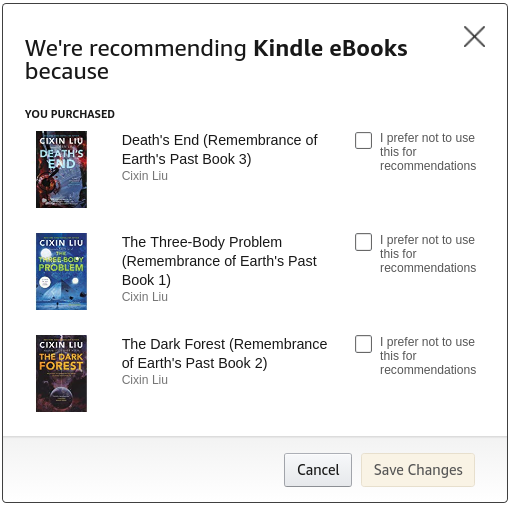
\includegraphics[scale=0.5]{img/AmazonExplanation.png}
    \caption{Amazon's web-page window that provides context why was a particular book recommended.}
    \label{fig:amazon_explain_book_recommendation}
\end{figure}

\begin{figure}[htbp]
    \centering
    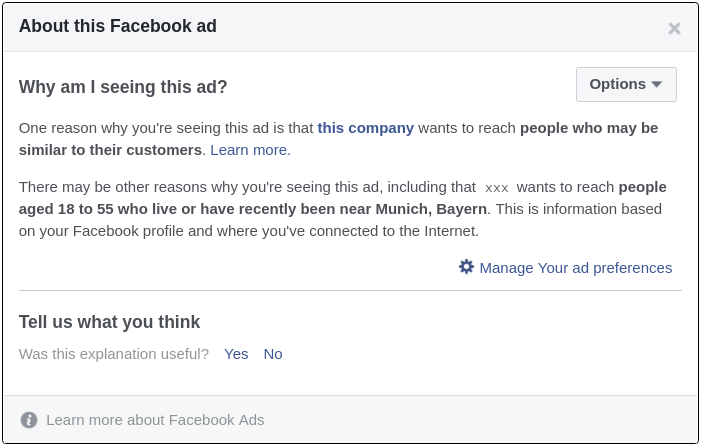
\includegraphics[scale=0.5]{img/FacebookAdExplanation2.png}
    \caption{Facebook's web-page window that provides information about what data lead to user's seeing Facebook's ads.}
    \label{fig:facebook_explain_book_recommendation}
\end{figure}

\subsection{Legitimacy}
Legitimacy can be viewed as an another step after explainability. When we provide a prediction together with a sound reasoning that can be verified either by a human analyst or by an other trusted system, then we can use it in more serious and sensitive deployments. One of them can be the legal domain. In it, computer systems can be used to provide unbiased and fair decisions and analysis, if set up correctly. But as mentioned many times before, we need to be very careful with the data that we use for training. Lot of care needs to be taken even if we do not use an automated training solutions. Most of the current systems used in the mentioned legal domain and other systems where legitimacy is required are most probably base on hand crafted rules that can very well be subject to bias as well. One of the examples being the system COMPAS presented in \ref{subsec:02_algo_fairness.examples_of_algo_biass}.

%\subsection{Auditability}
%\todo[inline]{Add 'Auditability?'}



\subsection{Consistency}
% \todo[inline]{Proc tahle uvodni veta? R: Protoze jsem to bouchal rychle jak hladovej datel :D :| a neprecetl si to po sobe.}
% \todo[inline]{tady vysvetli o jakou novelty ti jde - z kontextu bych tipoval, ze novelty ve smyslu davat na stejny input vzdy trochu jine doporuceni, protoze ty predchozi uz uzivatel videl, ale ani ja si tim nejsem jisty}

For some systems it is very important to stay consistent in outputs even with a slightly different inputs. Lets assume, that we are developing an illness detection algorithm, that offers medical personnel some insights about their patients based on provided symptoms. The predicted recommendation should not drastically change if for example the temperature changes by 0.1°C. It is therefore closely tied to the previous properties of legitimacy and explainability. Most high critical ML systems have to be designed with consistency in mind. Driver-less cars that abruptly change direction with only one pixel change in the input would not induce trust of its users.

From a different perspective we can view fairness as a sort consistency in the way that protected attributes of people do not have an effect on the output, the algorithm is consistent in respect of these protected attributes.
% \todo[inline]{Tady bys mohl zminit ze to souvisi i s fairness v tom ohledu, ze klicove protected atributy lidi by nemely mit vliv na vysledek -> alg. je vuci nim konzistentni. R: To je moc pekny osli mustek.} 

% From less high critical systems we can mention navigation properties in software and recommendation. We sometimes need machine learning user-tailored systems that are exceptional for speeding up work or retrieval of information, but its users would not be comfortable with often changes in the provided recommendations. 

One other meaning of consistency in regards to ML systems can be stability in the meaning of ML outputs being the same while navigating a system or an app. We can attribute it to the application's design more than the ML system it self. If a user is browsing a web page, lets say an aggregator of products on the web, they may rely on the back button while browsing the different outputs. In this setting, inconsistency and changes to the recommendation items may be harmful as it will affect the user experience while listing and using the provided information.

\subsection{Novelty}
Novelty can have multiple meanings when we use it to describe RS. Firstly it can be that the item it self is a new addition to the data-set and we do not have many user-item interactions which we would use to asses and recommend the new item.

Secondly, we can say that the the item is presented to the user for the first time. Sometimes, depending on the presentation of the recommended items, we have to show the recommended item repeatedly in order for it to be noticed. In that way, novelty can be viewed as a non binary attribute, where each time we present the item to the user it decreases the items novelty, with respect to that one user. But often it is viewed as a binary attribute, shown or not-yet-shown.

Thirdly, by novelty we can describe that an unusual item is presented to the user. Such situation can occur either due to the RS incorrectly assuming that the user will like that item, or by, on purpose introducing a new not yet seen item so that we introduce more exploration and present items that the user will view as fresh.

And lastly, novelty is important as an exploration. RS should try to broaden and expand the model of users' preference, which needs to be done by gathering feedback on items outside of the users current preference model. Balance between exploration and exploitation is difficult, but can substantially increase models' performance if done correctly.

In general and contrary to the previously mentioned consistency parameter, we usually strive for novelty and exploration. If a person is picking out a movie to watch, then showing them the same selection over and over would most certainly lead to their dissatisfaction due to the limited and repeated content that the system is providing. As with all properties, novelty requirements heavily depend on the domain the system is deployed in. This property is most sought for in domains where exploration is important.




% As an example, we can imagine that in a movie recommender system a user only watched Harry Potter movies, then a RS that does not try to introduce new novel items will only recommend other Harry Potter movies which will most probably be seen as boring, repetitive and valueless.


% 3 meanings
% new item in dataset
% new item presented to user
% unusual item presented to user
% item that wasn't shown to the user that many times



Contrary to the previously mentioned consistency parameter, we sometimes strive for novelty and exploration. If a person is picking out a movie to watch, then showing them the same selection over and over would most certainly lead to their dissatisfaction due to the limited and repeated content that the system is providing. This property is most sought for in domains where exploration is important.



% \todo[inline]{Zrovna pro novelty existuje celkem dost docela zajimavych interpretaci, ktere se daji zminit. Novelty jako inverse popularity (pokud nemame zaznamy o impressions, interakcni novelty - uzivateli jsme to zatim (mockrat) nezobrazovali, temporalni novelty - je to nove vytvoreny produkt}

\subsection{Coverage}
% Popsat situaci kde rs failuje v tom, ze nejake itemy jsou unreachable, nebudou pak doporuceny vsem, pripadne muzeme taky zminit to, ze popularni itemy budou vzdycky ve vyhode ktera nemusi byt uplne fair v tom, ze kdyz mas exposure tak je jednodussi dostat dalsi exposure, takovej trochu negative feedback loop. A muze se pak stavat, ze misto toho abychom doporucili item ktery je opravdu awesome pro toho uzivatele tak doporucime neco no neni tak awesome

In some ML and RS applications, there can emerge a situation where some items are never recommended. If the reason is that the item quality is bad then it can be the right system quality. In other situations, such as RS that recommends based on item properties, an undesirable behavior can occur when an item is just too different and we do not have a reasonable 'link' to other items that would serve as comparison for the recommendation. Then this item will be left out and never recommended.

Other coverage problem is with items that are popular. Popularity is sometimes a good indicator of quality, but not always. If an item is popular, then in a system that exploits popularity, it will receive more and more attention. This in turn further increases its popularity. In a way we can have a same type of phenomenon as Negative feedback loop mentioned in \ref{subsubsec:02_algo_fairness.adverse_effects.nfl}. It then happens that item exposure distribution will be unnaturally skewed even more towards the popular items. This can lead to decrease in system's performance due to some items that are less popular not being recommended even if being possibly a better choice for recommendation. In a way popularity and unpopularity correspond to a notion of novelty where instead of considering a single user we consider all users of the system together.

% \subsection{Diversity and similarity}
%

\subsection{Efficacy, accuracy and precision}
We have so far mentioned multiple other criteria. But all of them are hard to measure due to their somewhat subjective nature, let us now present two of the most widely used exact efficacy properties: accuracy and fairness.

Accuracy (sometimes as trueness) is a measure of how far away outputs of a ML system are from the desired outputs. Precision is a measure of how unsure or dispersed the outputs are, in other words how away are from each other. They are both measures of observation error and the definitions differ based on type of the systems outputs. We can see an illustration for continuous value prediction on \ref{fig:accuracy_fairness}

\begin{figure}[htbp]
    \centering
    \includesvg[width=9.5cm]{img/accuracy_and_precision.svg}
    \caption{Illustrative description of the relationship of accuracy and precision from \cite{Accuracy_precision}}
    \label{fig:accuracy_fairness}
\end{figure}

How to measure the distance of outputs to ground truth can differ based on the shape/dimensionality of the output. Usually we use a simple metric such as Euclidean distance or simple Manhattan distance.


For categorical data we have (binary retrieval task and multi-class classification respectively):
\begin{equation}
    Accuracy = \dfrac{\text{TP + TN}}{\text{TP + FP + TN + FN}} = \dfrac{\text{correct classifications}}{\text{all classifications}}
\end{equation}
and precision for binary classification:
\begin{equation}
    Precision = \dfrac{\text{TP}}{\text{TP + FP}}
\end{equation}

Precision for categorical data does not have a set meaning, we can either use precision for each class separately or have one class that act as a FP label.

Difficulties with using accuracy arise when miss labels to some or all items in the dataset. Calculating the correct denominator in categorical case or the correct distance to the reference value can be difficult or and impossible.

\subsection{Performance and scalability}
% Popsat motivaci teto sub, performance vice vyznamu, total resources needed, odezva, availability, scalability, one computer nezvladne uplne vsechno co si vymyslim
We can design any algorithm we want, but what for will it be if cannot then use it in the real world? Theoretical algorithms certainly have their place, but we are aiming to solve real problems of addressing fairness. Therefore another and last discussed property will be performance and with it related property of scalability.

Performance of as system can be described either in a form of total computational resources needed for processing, either the whole deployment or normalized to a single user. Other possible performance property can be the length of time needed for processing of a single request called latency. These two properties usually need to be balanced against each other. To a certain point we can either add more computational capacity to improve - decrease latency, or remove some capacity with the possible increase in latency.

Scalability is a property of a system that the it is able to handle a growing amount of work. We have to keep this property in mind while designing ML and RS systems. If for example we are using a comparison with other users such is the case in some RS algorithm, we will be growing the system requirements most probably linearly with the amount of users. This can be fine in for example research applications, but becomes a real concern when applying to a world wide applications used by millions of users. At these scales we will be required to scale using not only vertical scaling (that is using a more powerful computational resources), but mainly using horizontal scaling (by using many computers at once).



% \todo[inline]{Z toho co tu jsou jen jako nadpisy, tak diversity a similarity mi trochu splyvaji, podobne precision a accuracy - minimalne vzhledem k tomu ze jsi o ostatnich vecech mluvil na dost high-level urovni, tak bych tohle asi spojil dohromady.}


% TODO: Fairness is not the only property we can try to manage, what about privacy, accuracy, precision, coverage, diversity, novelty and so on. Mention them first in an overview, then separately in subsections in more detail. Try to define them mathematically.
